show the extent to which there is true monosemanticity within features by interp across full activation range

autointerp on the lowest quintiles 


\subsection{Detailed feature analysis}
Here we show that features seem quite interpretable, look at lower activation levels, monosemanticity

\subsection{Building graphs!}
Look we can build graphs of features which makes sense
Can we at least qualitatively show that this doesn't work well with neuron basis?
(or PCA basis or something for the residual)


\subsection{Finding features}
Can we do checks for whether features are explainable in terms of other features?
One test is we try to decompose features into simple combinations of other features. if it turns out we can recreate the meaning of the feature from the composition of the meanings of the separate features then now we're perhaps not seeing superposition but just composition of features. would expect to see it more strongly as we increase the dictionary size. also do we find the separate but not compositr in smaller dicts

\subsection{circuits at scales}
look for roughly the same circuit in two models of different sizes, e.g., what's causing a close paren, see if we can see interesting differences

look at the capacity measure for neurons, see the distribution maybe look at low capacity as evidence for starting to have too many feats \citep{scherlis2023polysemanticity}

\subsection{causal alignment geiger}
geiger lots of work showing causal abstraction is an important desiderata for whether we have succeeded in understanding a network with our high level understanding\citep{geiger2023causal}
can we calculate measures of abstractability that measure our ability to breakdown networks of calculation, use this to score differences between building graphs with neuron basis/pca/resid basis/ica








\subsection{clustering results}
[Question from Robert: What experiment did we run in this section? What were the results?]

can cluster the dictionary elements, show that they get similar autointerp results, sometimes district, sometimes not on autointerp, later will show that tend to be distinct, further analysis in subsequent section

\section{topk}
\label{appendix:topk}

\section{Other Appendices?}
Cool stuff that didn't go elsewhere
additional demonstration in appendix of similarity 
can we do just the exact 

more dict sizes, draw frontier as you increase, compare to synth

methods for checking dict size

characterise the weaknesses of the autointerp method


\section{Analysis}
Try to understand what it is about these dictionaries that are making them interpretable
doesn't seem to be that strongly about the ability to sparsely reconstruct, see aidan graph using topK pca

on the otherhand, some evidence that even when we set the l1 coefficient to zero, it still outperforms the neuron basis and pca (kinda mad!) 

\begin{figure}
    \centering
    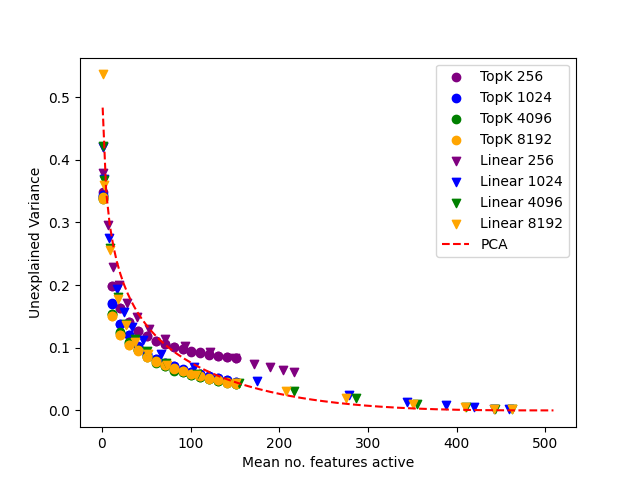
\includegraphics[scale=0.4]{images/pca_plot_place.png}
    \caption{applying top-k filtering to PCA directions gives a similar tradeoff between sparsity and unexplained variance  - but this doesn't translate into interpretable directions}
    \label{fig:pca_plot_place}
\end{figure}


